\section{Does OPD Expand Student's Capability Boundary?}
\label{sec:opd_phenomena}


The implicit-reward perspective suggests that successful OPD can improve performance by reinforcing correct student responses.
We examine this successful case: does teacher feedback make problems already solvable by the initial student easier to solve?
We compare the initial student \(S_{\mathrm{INIT}}\) with the trained student \(S_{\mathrm{OPD}}\) using \(\mathrm{pass}@k\) across increasing sampling budgets, audited problem coverage, and per-problem success rates.



\paragraph{Gains diminish as the sampling budget grows.}
\label{sec:3_1}
\begin{figure*}[t]
    \centering
    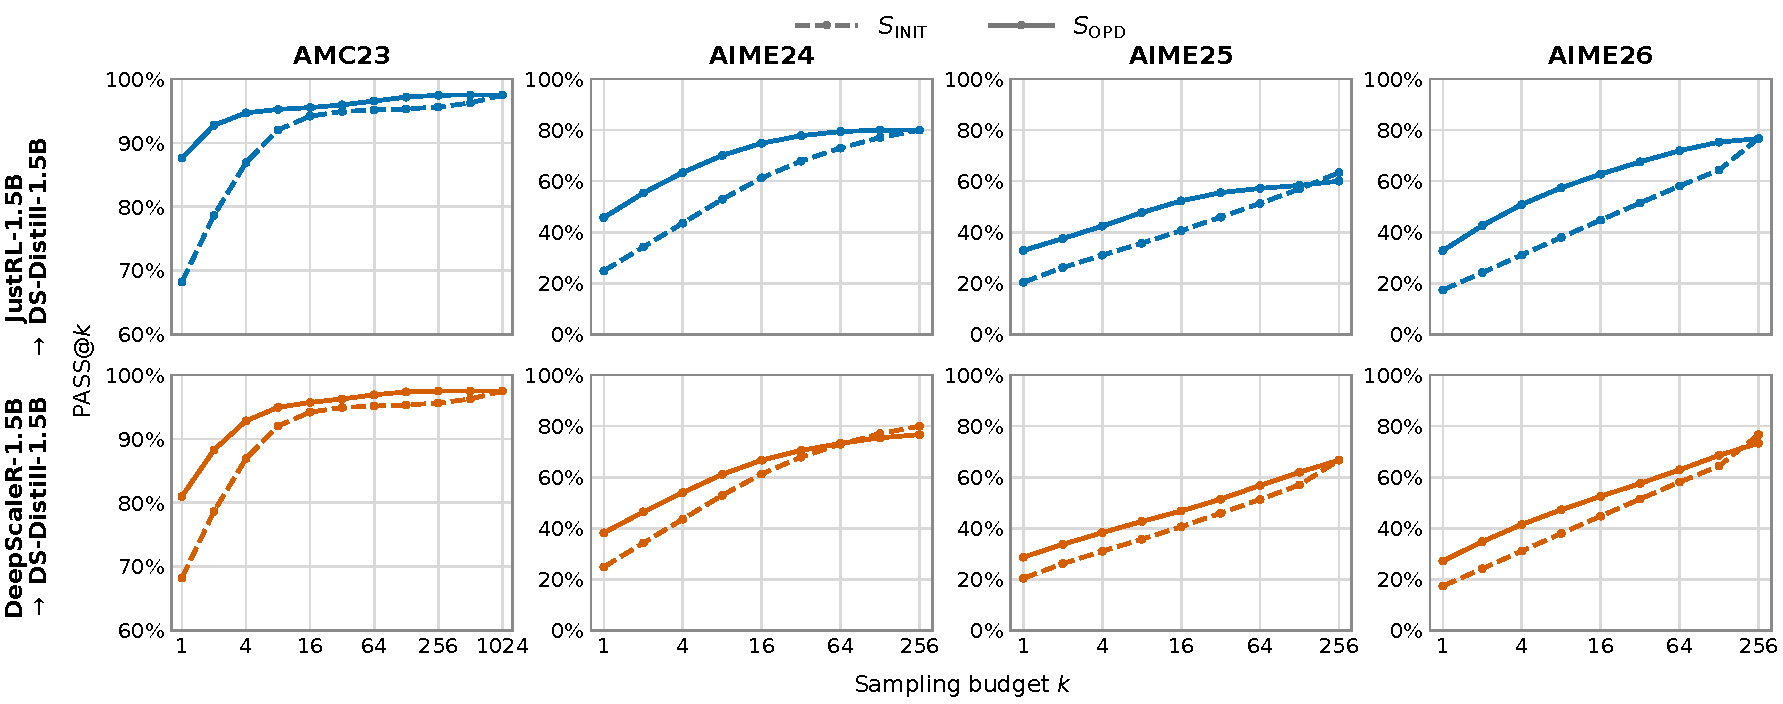
\includegraphics[width=0.98\textwidth]{S3/dsr_s3_pass_at_k_mpl.pdf}
    \caption{
        \textbf{\passk{k} curves of \(S_{\mathrm{INIT}}\) and \(S_{\mathrm{OPD}}\).}
        Across AMC23 and AIME24--26, OPD gains are largest at small \(k\) and
        shrink as the sampling budget grows. AIME curves extend to \(k=256\),
        while AMC23 extends to \(k=1024\).
    }
    \label{fig:s3_sampling_accuracy}
\end{figure*}

We compare the initial student \(S_{\mathrm{INIT}}\) with the trained student \(S_{\mathrm{OPD}}\) under both teachers, JustRL-1.5B and DeepScaleR-1.5B-Preview, on AIME24--26 and AMC23.
We compute \passk{k} from each response pool for \(k\in\{1,2,4,8,16,32,64,128,256\}\) on AIME and additionally \(k\in\{512,1024\}\) on AMC23, averaged across all test cases.


As shown in Figure~\ref{fig:s3_sampling_accuracy}, we observe a consistent trend under both teachers.
When \(k\) is small (e.g., \(k=1\), equivalent to average-case accuracy), \(S_{\mathrm{OPD}}\) clearly outperforms \(S_{\mathrm{INIT}}\).
However, as \(k\) increases, \(S_{\mathrm{INIT}}\) steadily catches up.
At the maximum available \(k\), \passk{k} equals the observed coverage: the fraction of problems solved at least once in the response pool.
This suggests that OPD improves accuracy under a small sampling budget, but does not improve the observed coverage at higher \(k\).



\paragraph{No Observed Expansion in Problem Coverage After OPD.}
To distinguish new coverage from finite-sample misses, we first identify the problems solved by $S_{\mathrm{OPD}}$ but not by $S_{\mathrm{INIT}}$ within the original 256-response pools of AIME24-26.
For each of these problems, we draw 768 additional responses from \(S_{\mathrm{INIT}}\), bringing its pool to 1024 responses.
Manual review checks derivation validity and corrects verifier misses in the existing outputs.


\begin{wrapfigure}{r}{0.5\textwidth}
    \centering
    \vspace{-5mm}
    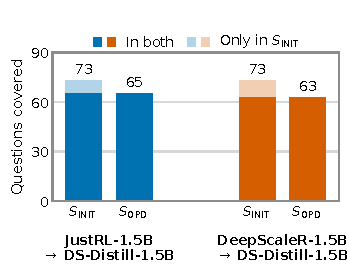
\includegraphics[width=0.85\linewidth]{S3/coverage_bars_mpl.pdf}
\captionsetup{font=footnotesize}
    \caption{
        \textbf{Change in observed coverage from \(S_{\mathrm{INIT}}\) to \(S_{\mathrm{OPD}}\).}
        No problem is solvable by \(S_{\mathrm{OPD}}\) but not by \(S_{\mathrm{INIT}}\) in our observation.
        Counts come from the audited pools with conditional extension to 1,024
        responses.
    }
    \label{fig:s3_coverage_partitions}
    \vspace{-7mm}
\end{wrapfigure}

After additional sampling and manual review, no problem remains solved only by
$S_{\mathrm{OPD}}$: candidate cases are resolved either by finding a valid
$S_{\mathrm{INIT}}$ solution or by excluding an invalid $S_{\mathrm{OPD}}$
derivation. The audited $S_{\mathrm{INIT}}$ set contains 73 solvable problems,
against which $S_{\mathrm{OPD}}$ covers 65 under JustRL-1.5B and 63 under
DeepScaleR-1.5B-Preview. These counts are larger than the $k=256$ endpoints of
Figure~\ref{fig:s3_sampling_accuracy}, which are computed before the audit.
Detailed coverage analyses are provided in Appendix~\ref{app:coverage_records}.
These indicate that OPD does not induce an observed expansion of the solvable set.



\paragraph{Already-solvable problems become easier to solve.}
\label{sec:3_3}

\begin{wrapfigure}{r}{0.5\textwidth}
    \centering
    \vspace{-5mm}
    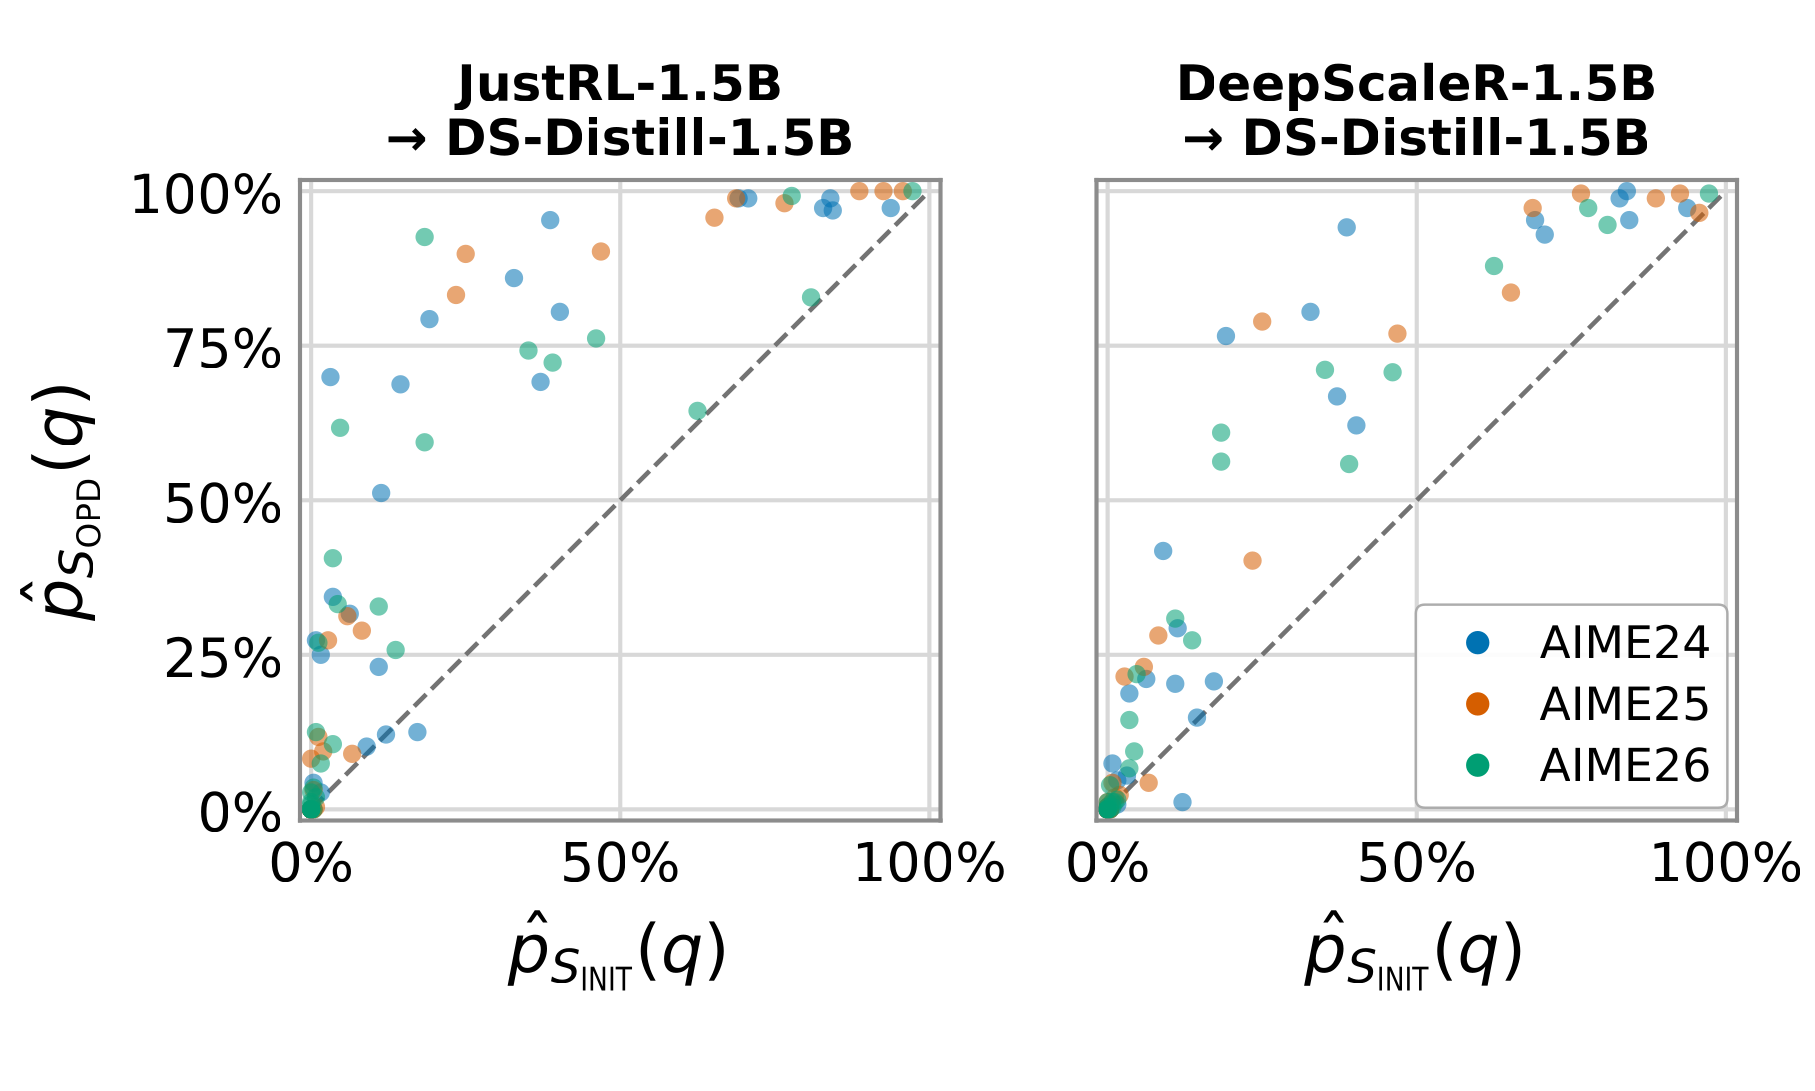
\includegraphics[width=\linewidth]{S3/sampling_efficiency_mpl.png}
\captionsetup{font=footnotesize}
    \caption{
        \textbf{Per-problem mean@256 of \(S_{\mathrm{INIT}}\) ($x$-axis) and \(S_{\mathrm{OPD}}\) ($y$-axis).}
        OPD raises success rates on problems already solvable by \(S_{\mathrm{INIT}}\).
        The dashed line marks equal score.
    }
    \label{fig:s3_sampling_efficiency}
    \vspace{-5mm}
\end{wrapfigure}

To identify the source of OPD's small-\(k\) gains, we compare per-problem success rates between \(S_{\mathrm{INIT}}\) and \(S_{\mathrm{OPD}}\).
For each problem \(q\), let \(\hat{p}_m(q)\) denote the fraction of correct responses among the 256 samples from model \(m\).



As shown in Figure~\ref{fig:s3_sampling_efficiency}, the problem-level distribution is strongly shifted above the diagonal under both teachers.
OPD increases the per-problem success rate for 90.6\% of the problems already solvable by $S_{\mathrm{INIT}}$ with JustRL-1.5B as the teacher, and for 84.4\% with DeepScaleR-1.5B-Preview.
Averaged over these problems, the increase in mean@256 is 22.6\% and 14.7\%, respectively.

Problems unimproved by OPD are those that \(S_{\mathrm{INIT}}\) could hardly solve, and no high-performing problem drops to near-zero accuracy (lower-right corner).
Some even jump from low to high success rates (upper-left corner), showing that OPD can make problems the initial student rarely solves much easier to solve.
Thus, OPD primarily eases sampling of correct answers on already-solvable problems, which accounts for the small-k performance gain.

\paragraph{Summary.}
In the two successful settings studied here, OPD improves sampling efficiency on problems already solvable by the initial student.
Its positive accuracy gains disappear at the largest sampling budgets tested, and no validated OPD-only problem remains after the targeted AIME coverage audit.
These findings are consistent with the teacher acting as an implicit reward model whose feedback reinforces correct student behavior, making successful responses easier to sample.
